\section[Experimental system for \tgfbsf/Wnt integration]{An endogenous system for studying \tgfbsf/Wnt crosstalk}
\label{insulation:system}




  \begin{figure}[!bt]
  \centering
  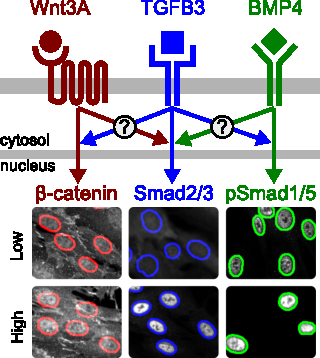
\includegraphics[width=3in]{FIGS/insulation/schematic.pdf}
  {\singlespacing 
  \caption[Schematic of the experimental system for \tgfbsf/Wnt crosstalk.]
        {Schematic of the experimental system for \tgfbsf/Wnt
         crosstalk. To measure inter-pathway signaling crosstalk,
         ligands can be applied combinatorially, followed
         by measurement of nuclear transcription
         factor levels. As shown, Wnt3A increases global
         quantities of \bcat, \tgf 3 causes translocation
         of bulk Smad2/3 to the nucleus, and levels of nuclear
         phospho-Smad1/5/8 increase upon BMP4 treatment.
         HCECs, with (``High'') or without (``Low'') 2hr treatment by
         Wnt3A (240ng/mL), \tgf 3 (4ng/mL), or BMP4 (73ng/mL).
         Outlines are of nuclei, segmented from the Hoechst channel
         (channel not shown) using the same threshold-segmentation method
         as in all imaging studies in this chapter.
         Fields are chosen to demonstrate visually obvious
         outcomes of signaling, though the diversity of responses
         is quite high for all pathways
         (see Figs. \ref{fig:insulation:ligandInformation} \&
         \ref{fig:insulation:readoutInformation}).}
  \label{fig:insulation:schematic}}
  \end{figure}
  

I reasoned that, because transcription factor activity is
the direct endpoint of signal transduction, I can infer the
degree of meaningful \tgfbsf\ and Wnt signaling interaction by measuring
how stimulation of one pathway affects the immediate transcription factor
response of the other pathway (\ar{fig:insulation:schematic}).
Current studies typically rely on transcriptional readouts to infer
such interactions, but these inferences may be confounded by transcriptional
feedback (which I consider to be the result of nuclear decision-making,
not signal transduction). Therefore, to accurately interpret cross-pathway effects
with respect to signaling, I use experimental timepoints that are
as close to the initial signaling event as possible.
Additionally, it is widely
believed that both Wnt and \tgfbsf\ signaling can be highly context-dependent.
I therefore repeat the experiments in this chapter using multiple
cell types, chosen to represent divergent cellular contexts.
By doing so, the hope is that any resulting shared properties of signal
integration can be more confidently extrapolated to other cellular systems.

In order to rigorously quantify single-cell responses to the
many experimental conditions required for this study,
and to make use of the expertise within the Altschuler \& Wu
lab, I use high-throughput immunofluorescence imaging as my primary
experimental platform. Unless otherwise indicated,
the presented measurements in this chapter originate from the
total-intensity feature values of individual nuclei. I typically report the
population-medians of these single-cell values, from replicate experimental
setups (as shown schematically
in \ar{insulation:system:measurement}; see \ar{imaging:introduction}
for more detail on my approach to image analysis).


  \begin{figure}[!bt]
  \centering
  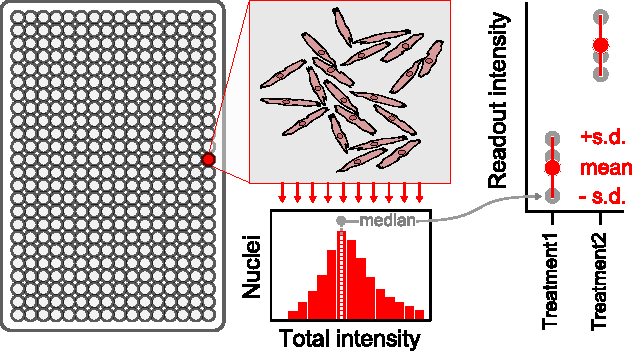
\includegraphics[width=3in]{FIGS/insulation/measurementSchematic.pdf}
  {\singlespacing 
  \caption[Schematic of the population-level fluorescence metric.]
        { 
        The fluorescence intensities reported in this
        chapter are population-level, based on single-nuclei
        measurements. As shown schematically here,
        cells are treated in
        96- or 384-well plates (left) and then fixed, immunostained,
        and imaged (middle, top).
        Nuclei are then identified computationally
        (see \ar{imaging:features}) so that the distributions
        of single-nuclei total fluorescence are obtained
        (middle, bottom). The medians of these distributions are
        then calculated for each replicate well. The reported
        values in this chapter are the means and standard deviations
        of these median values, nearly always from $n$=3 replicates.
        P-values are then calculated using an unpaired, two-tailed
        Student's t-test, and significant differences (p<0.05) are
        indicated with an asterisk. Figure legends indicate
        which samples are being compared for
        statistical significance.
        }
  \label{insulation:system:measurement}}
  \end{figure}
  

\subsection{Choosing cell types}
\label{insulation:system:readouts}


In order to choose useful cell lines, ligands, and readouts
for the study of Wnt and \tgfbsf\ signaling, I was confronted
with something of a chicken-or-the-egg problem. However, ongoing work
within the Altschuler \& Wu 
lab had made use of purified recombinant \tgf 1 for stimulating
the \tgf\ pathway and a total-Smad2/3 antibody for measuring the response.
Additional work had shown the efficacy of a \bcat\ antibody for
measuring cellular responses to purified Wnt3A. I therefore first made
use of these reagents, using literature-supported concentrations,
to identify cell lines that show responsiveness
to these pathways.


  \begin{figure}[!bt]
  \centering
  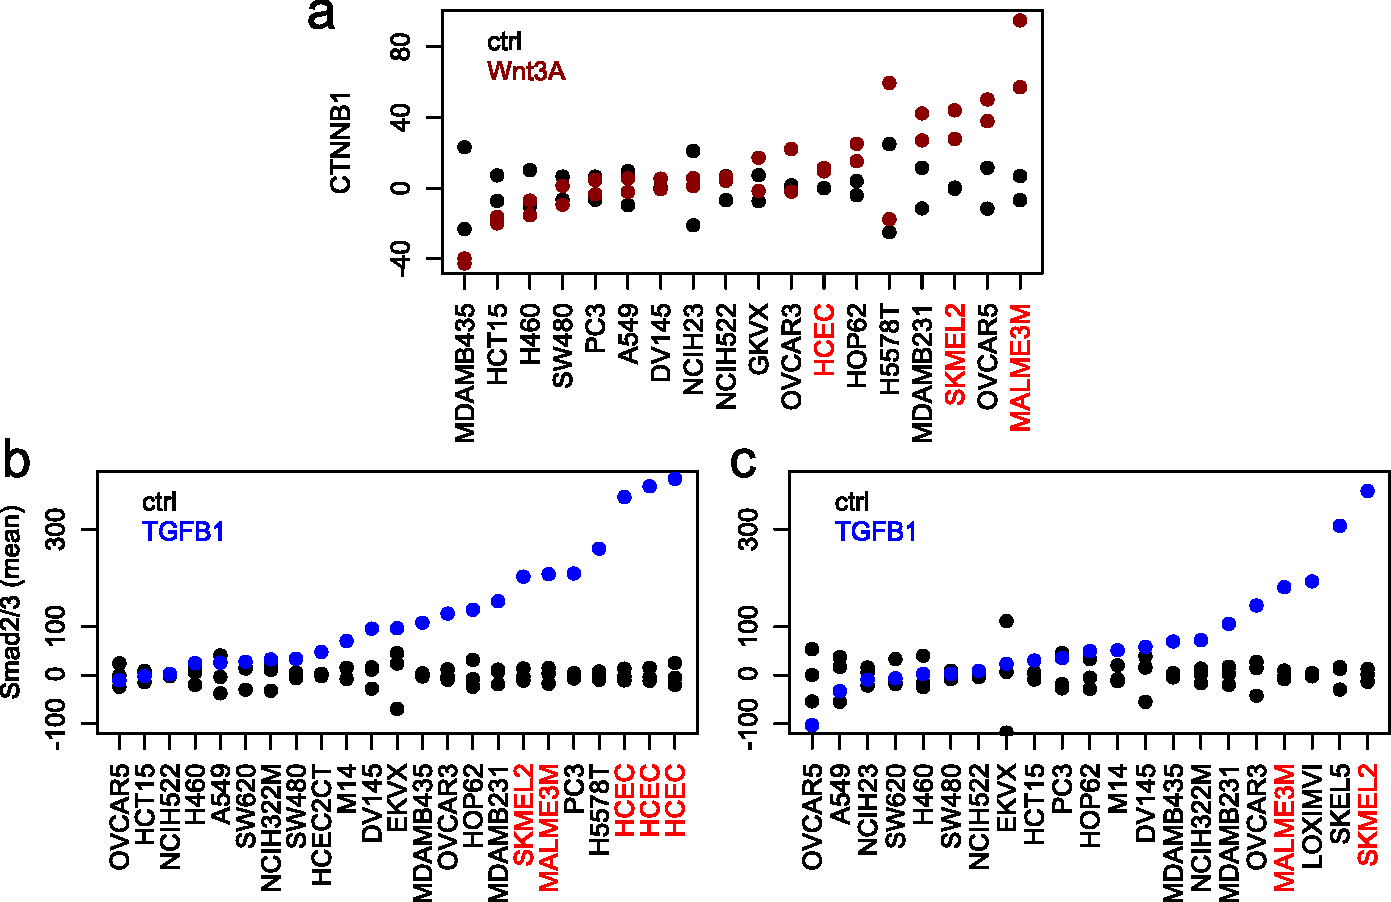
\includegraphics[width=6in]{FIGS/insulation/celltypeScreen.pdf}
  {\singlespacing 
  \caption[A screen for Wnt and \tgf\ responsive cell lines.]
        { A screen for Wnt3A (\b{a}) and
          \tgf 1-responsiveness (partial-replicate screens
          \b{b} and \b{c}) 
          across $\sim$20 cell lines revealed consistent
          responses by human colonic epithelial
          cells (HCECs) and two melanoma lines
          (SKMEL2 and MALME3M), highlighted with bright red text.
          The measured single-cell feature is the nuclear
          mean of fluorescence intensity by imaging
          (arbitrary units). Plots show the median
          of these single-cell values across all cells in
          a treated well (as in \ar{insulation:system:measurement}).
          The control means are subtracted from all values, per cell line,
          to show absolute changes in nuclear intensity.
          Concentrations: 1ng/mL \tgf 1, 200ng/mL Wnt3A.
          Timepoints: 1.25hrs (Wnt3A), 1hr (\tgf 1).
        }
  \label{fig:insulation:celltypeScreen}}
  \end{figure}


I first selected an immortalized (via telomerase and CDK4 expression)
but non-transformed human colonic epthelial cell (HCEC) line. This
cell line has stable ploidy and properties consistent with it being
a pseudo-differentiated cell type \cite{Roig2010}. Given the importance
of Wnt and \tgfbsf\ signaling in the gut (\ar{pathways:wntTgfb:gut}),
this cell line makes for a
reasonable model system for studying crosstalk between these pathways.
As a control, I also chose the rat small intestine
epithelial line (IEC6) \cite{Quaroni1978},
reasoning that it should display similar properties to HCECs.
I found that both of these
cell types respond strongly (in a statistical sense)
to TGFB ligands, moderately to BMP4,
and weakly (but measurably) to Wnt3A.


As discussed in \ar{introduction:encoding:context}, signaling
pathways generally show context-dependency, especially with respect
to differences in cell type. This non-generality is especially
true of the \tgfbsf\ and Wnt pathways (\ar{pathways:introduction}).
Therefore, in order to discover general properties (if indeed they exist)
we need to look for commonalities across cell types; the two intestinal
cell lines chosen may not be sufficient to infer generality. 
One approach to increase generality would be to
exhaustively test a large number of cell types, so that with each
successive cell type we gain confidence in the generality of a biological
phenomenon. Unfortunately, this approach is costly and difficult, and still
does not lead to certainty in the generality of a discovered phenomenon.
I opted then for a simpler approach, which is to test a small number of
divergent cell types. In this way, any behaviors consistent
across cell types can still be extrapolated as ``general'' behaviors,
though the resulting confidence in such a generalization may be somewhat
lower. 


To identify additional cell types for studying \tgfbsf\ and Wnt
crosstalk, I screened a panel of cancer cell lines for responsiveness
to \tgf 1 and Wnt3A. 
Additional selection criteria included cell morphology and
growth patterns that would allow for accurate image segmentation (see
\ar{imaging:features}), as well as cellular
growth rates and adherence properties that would
allow for the throughput needed for the many experimental conditions
required in my studies.
Two melanoma cell lines, SKMEL2 and MALME3M,
satisfied these criteria and were consistently ranked among the most
responsive to both \tgf 1 and Wnt3A (\ar{fig:insulation:celltypeScreen}).
Both of these cell lines can form malignant melanomas in nude mice, and
have abnormal ploidy  \cite{Fogh1977}. In particular, I found that SKMEL2 cells always
form tri-modal cell cycle distributions, implying the presence of diploid,
tetraploid, and octoploid cells within an asynchronous cycling population.
To my knowledge, there are no Wnt or \tgfbsf\ pathway mutations in SKMEL2
or MALME3M cells.


These cell lines should not be used to make
inferences with respect to differences between ``normal'' and cancer
cells, as these cell lines differ also in tissue of origin. Instead,
they should be thought of simply as divergent pairs of cell types that provide
consistent ``contexts'' (e.g. within the two intestinal lines or
within the two melanoma lines ) as well as divergent contexts (e.g.
between the intestinal and melanoma lines).
For all analyses in this chapter, I use only those cells
within the first peak of the imaging-based cell cycle distributions
(see \ar{imaging:variation:dnaQC}). I verified for each individual
pathway that the position of a cell within the cell cycle distribution
was not predictive of pathway behavior (data not shown) and
restriction to the G1/0 cell cycle phase otherwise reduces both experimental noise and
unimportant biological variation.
  
  
\subsection{Choosing signaling inputs and outputs}
\label{insulation:system:inputOutput}


Having chosen the cellular contexts in which to measure
the signaling crosstalk between \tgfbsf\ and Wnt, I then
needed to choose inputs and outputs that
could be believably interpreted to represent these pathways.
As discussed in \ar{introduction:encoding}, as a rule it
is not known what aspects of a signal or a readout are the
most relevant carriers of information for a cell. It is
generally believed, however, that for morphogenic pathways
it is the extracellular concentration of a ligand and the
nuclear concentration of a corresponding transcription factor that
are the relevant parameters. I therefore tested several ligands and readouts
in order to identify experimental inputs and outputs that are
both meaningful and practical.


  \begin{figure}[!bt]
  \centering
  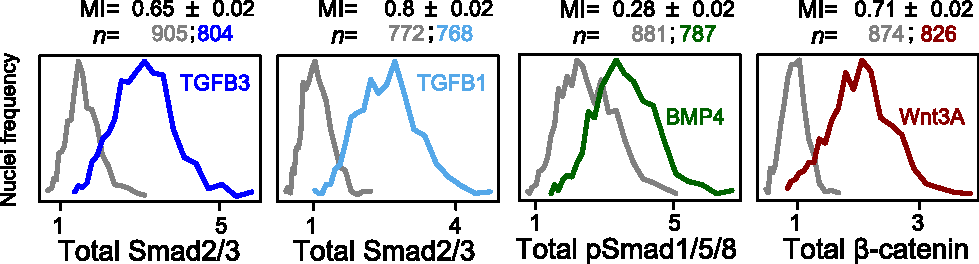
\includegraphics[width=6in]{FIGS/insulation/ligandInformation+.pdf}
  {\singlespacing 
  \caption[Information content of experimental treatments.]
        { Saturating ligand concentrations of \tgf 1/3 (12ng/mL), 
          Wnt3A (730ng/mL),
          and BMP4 (8ng/mL) are informative with respect to
          their canonical
          transcription factors. MI,
          mutual information between the ligand and readout
          (in bits, maximum MI is 1, see \ar{imaging:information}). 
          Histograms, distributions
          of single-cell total nuclear intensities for the
          immunostained transcription factors. $n$, number of cells
          per histogram, pooled from 3 replicate wells 
          (color-coded). Gray, untreated. 
          SKMEL2 cells, 1hr treatment. Arbitrary fluorescence units,
          frequencies scaled to have the same maximum value for display
          purposes.}
  \label{fig:insulation:ligandInformation}}
  \end{figure}
 
\subsubsection{Choosing prototypical ligands}
 
I first assayed several pathway inputs for information
content and signaling specificity. For the BMP2/4 pathway, I found that
all cell lines were non-responsive to purified BMP2 (data not shown) but
responsive to purified BMP4. These two ligands are
highly homologous and are thought to act through the same receptors
(\ar{pathways:tgfb:ligands}) therefore this absence of effective BMP2
signaling does not have a clear interpretation (perhaps a faulty reagent). In any event, the 
BMP4 signal is informative (using the mutual information metric,
as described in \ar{imaging:information});
the distribution of single-cell responses to saturating BMP4 is wide
but significantly different from the control distribution 
(\ar{fig:insulation:ligandInformation}). 


For the \tgf\ pathway I compared \tgf 1 and \tgf 3, as these ligands
are considered to be essentially interchangeable
(\ar{pathways:tgfb:ligands}). Indeed, within a single experiment
these two ligands generated similarly broad and separated Smad2/3
responses with similar mutual information
(\ar{fig:insulation:ligandInformation}). Dose-response curves for
the two ligands have the same
maxima and similar hill coefficients, though \tgf 3 is $\sim$10 time more
efficacious than \tgf 1 (data not shown).
\tgf 3 generally yielded more reliable responses, and so I use this
ligand for the remaining experiments in this chapter.


Finally, I chose to use purified Wnt3A to stimulate the canonical
Wnt pathway. Wnt3A is considered the prototypical ligand for this
pathway (\ar{pathways:wnt:wnt}), and its commercially-available
purified form has been widely used throughout the literature.
Importantly, I discovered that what is likely the most
commonly-used form, a low-purity ($\sim$75\%)
version from R\&D Biosystems, is sufficient to send Smad2/3 to the nucleus with the same
kinetics and dose-response Hill coefficicent as seen with \tgf\ treatment
(\ar{fig:insulation:contamination}a). I was unable to measure contaminating \tgf\ ligands
by Western (\ar{fig:insulation:contamination}b),
though this could be due to low concentrations of a high-efficacy \tgf\ variant.
In any event, this pathway crosstalk is likely
a consequence of trace amounts of contaminating \tgf\ in
the purified Wnt, as a pan \tgf-blocking antibody is sufficient to
block this response. Further, high-purity and carrier-free variants of the
product do not activate Smad2/3 (\ar{fig:insulation:contamination}c).


This artifactual crosstalk also occurs with the prototypical non-canonical
Wnt5A (\ar{fig:insulation:contamination}a,c), which casts
uncertainty onto recently-published work
linking Wnt5A and \tgf\ signaling
(reviewed in \ar{pathways:wntTgfb:dvl}) \cite{Miyoshi2012}.
The presence of such contamination may complicate the
interpretation of many other published studies, as it
suggests that treatment with purified Wnt3A or Wnt5A may generally include treatment
with \tgf, such that some resulting phenotypes 
could be due to stimulation by Wnt, \tgf,
or both.


  \begin{figure}[!bt]
  \centering
  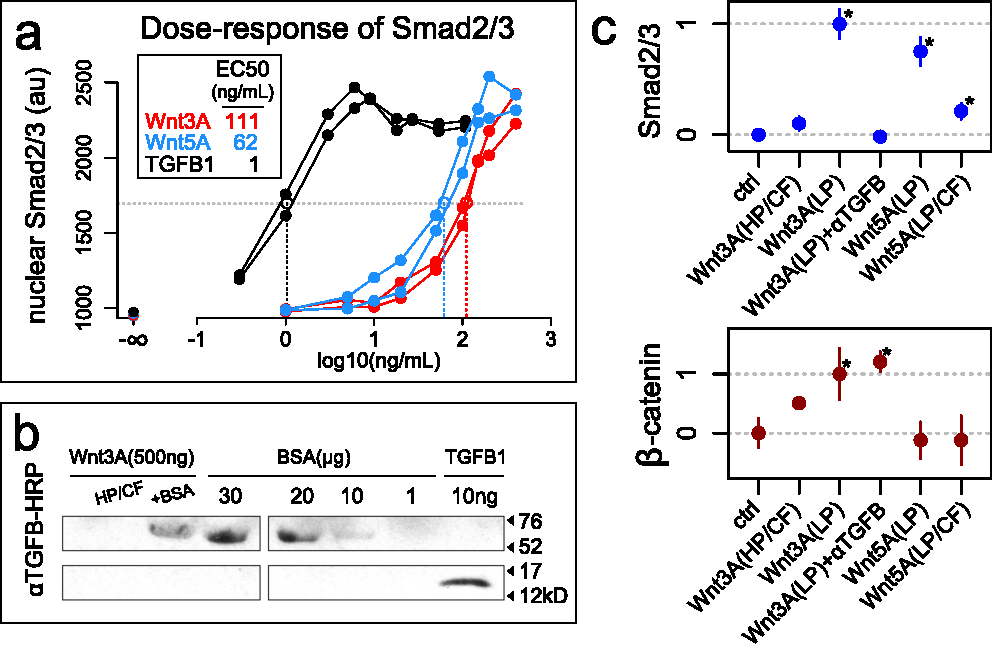
\includegraphics[width=5in]{FIGS/insulation/contamination+.pdf}
  {\singlespacing 
  \caption[Contamination of commonly-used commercial Wnt3A.]
        { The commonly-used low-purity (75\%) Wnt3A and Wnt5a ligands have
          trace amounts of contaminating \tgf.
          \b{a}, Dose-response curves
          for Wnt3A and Wnt5A against Smad2/3 yield EC$_{50}$ concentrations for
          the Wnts that are comparable to those used in the literature
          to stimulate Wnt responses (>100ng/mL is common).
          Duplicate experiments. Median of the mean nuclear
          intensity is plotted for each well (as in \ar{insulation:system:measurement}).
          \b{b}, Western blot of
          the purified Wnt3A ligands using a pan-\tgf\ antibody. HP/CF
          is the high-purity/carrier-free ligand used throughout this
          chapter, +BSA is the low-purity Wnt3A. BSA is shown as a reference.
          The low-purity Wnt3A lane should contain
          $\sim$25\textmu{g} of BSA in this blot, which is enough protein
          to soak up significant \tgf\ antibody.
          \tgf 1 is $\sim$12 kiloDaltons.
          \b{c}, The apparent Wnt$\rightarrow$Smad2/3 response is completely blocked
          by co-treatment with a pan-TGFB antibody that does
          not block the ability of Wnt3A to stimulate a \bcat\
          response. Low-purity Wnt5A also stimulates Smad2/3,
          but a carrier-free (CF) version does not. The high-purity (>90\%)
          carrier-free (HP/CF) Wnt3A shows a minimal Smad2/3
          response that is reproducible in other experiments, though not significant
          in this one. Concentrations: Wnt3A (200ng/mL),
          Wnt5A (100ng/mL), \textalpha{TGFB} (5\textmu{g}/mL).
          Y-axes and p-values as in 
          \ar{fig:insulation:specificity}.
          \b{a,c}, HCECs, 1hr treatment.}
  \label{fig:insulation:contamination}}
  \end{figure}

  
I therefore use high-purity/carrier-free Wnt3A for all experiments
in this chapter. I note, however, that even this ligand often causes
a small increase in Smad2/3 and so crosstalk experiments must be
interpreted with this fact in mind.

  
\subsubsection{Choosing prototypical readouts}


Having identified robust pathway inputs, I then needed to validate
antibody-based pathway outputs for immunofluorescence imaging.
For the \tgf\ pathway, which specifically activates Smad2/3,
and the BMP4 pathway, which specifically activates Smad1/5/8
(see \ar{pathways:tgfb:smads}),
I find that the nuclear fractions of both active phospho-protein and
total-protein levels can respond robustly to pathway activation.
However, it is unclear from the literature whether it is the total
concentration or the phospho-state concentration that encodes
extracellular ligand levels.


  \begin{figure}[!bt]
  \centering
  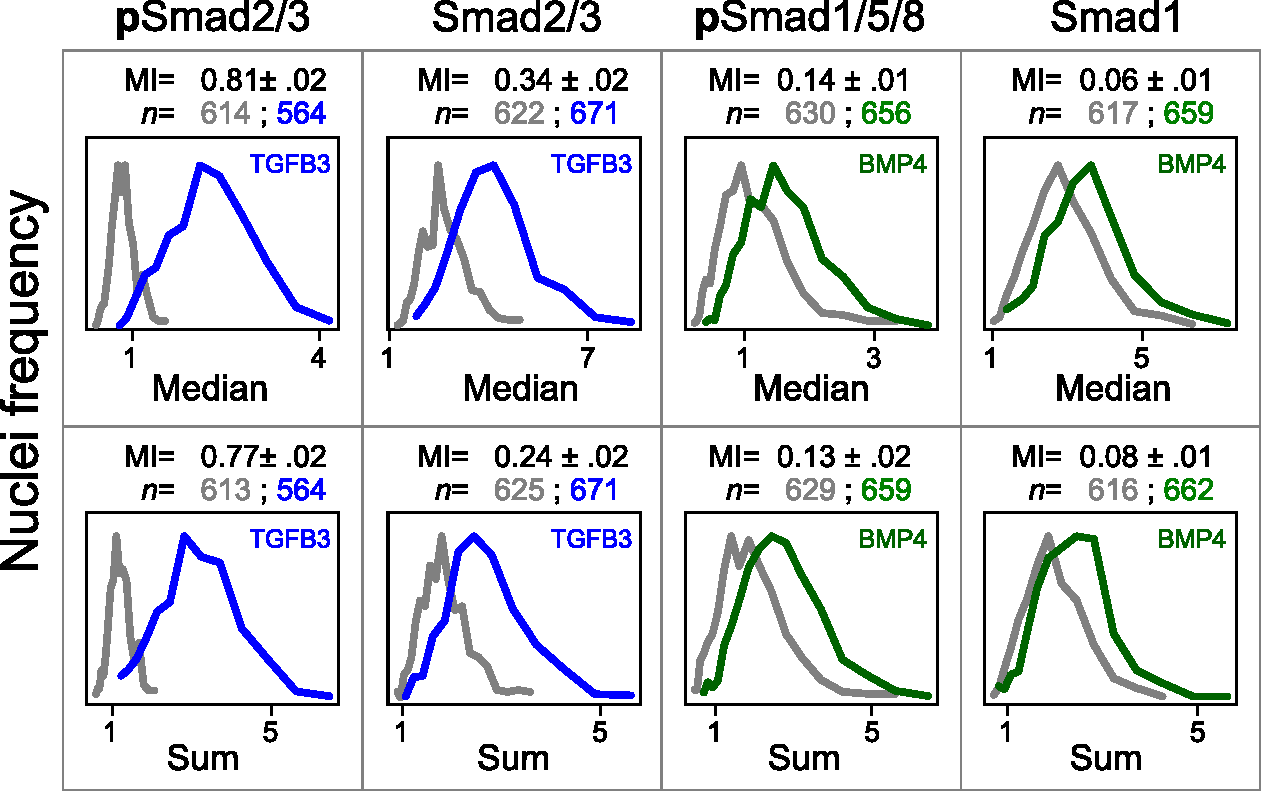
\includegraphics[width=5.5in]{FIGS/insulation/readoutInformation+.pdf}
  {\singlespacing 
  \caption[Information content of Smad readouts.]
        { Nuclear phospho-Smads (pSmads) contain more information about
          ligand concentrations than do nuclear total-Smads,
          though the sum and mean of intensity features are comparable. The
          untreated (gray) and treated (colored) distributions
          of single-nuclei measurements show more overlap
          of total-Smad readouts, resulting in relatively less mutual
          information (MI, in bits, maximum of 1, see \ar{imaging:information}).
          The median (top row) and
          sum (bottom row) of nuclear intensities for a single readout
          have nearly identical information content.
          $n$, number of cells
          per histogram (color-coded). 
          Ligand concentrations: saturating 10ng/mL
          \tgf 3 (blue) or 50ng/mL BMP4 (green).
          SKMEL2 cells, 1.5hr treatment. Arbitrary fluorescence units,
          frequncies normalized to have same maximum value.}
  \label{fig:insulation:readoutInformation}}
  \end{figure}


I therefore measured the mutual information
between these readouts and their ligands, which
revealed that the phospho-state is indeed more informative
(\ar{fig:insulation:readoutInformation}). Care should be taken when
interpreting this data, however, as the difference in information content
may also be due to antibody specificities, along with a myriad of
other causes. I note that
I have never observed maximum mutual information values of more than $\sim$1.2 bits
for any type of input/output relationship from imaging data, consistent
with published reports \cite{Cheong2011}.
The most fair statement, then, is that these particular approximations
of the phospho-state are more informative than these approximations of
total protein levels.


The total-Smad2/3 antibody yielded more-consistent
results across experiments than did the phospho-Smad2/3 antibody,
however, and has similarly-high
information content. I therefore use the total-Smad2/3
and the phospho-Smad1/5/8 (pSmad1/5/8) antibodies for the crosstalk experiments.
For canonical Wnt signaling there is strong evidence that it is the
total-protein level of \bcat, not the phospho-state, that encodes ligand concentration
(\ar{pathways:wnt:bcat}). I therefore use a total-protein \bcat\ antibody
to measure canonical Wnt responses.


\subsubsection{Validating input/output relationships}



  \begin{figure}[!bt]
  \centering
  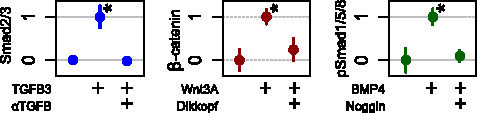
\includegraphics[width=4.5in]{FIGS/insulation/specificity+.pdf}
  {\singlespacing 
  \caption[Specificity of ligand/transcription factor relationships.]
        { The measured canonical transcription factor responses are a specific
          consequence of ligand treatment. \b{Left}, A
          pan-TGFB antibody (\textalpha{TGFB})
          blocks 2hr \tgf 3-induced
          nuclear Smad2/3 accumulation in HCECs. \b{Middle},
          Dikkopf, a soluble antagonist (\ar{pathways:wnt:frizzled}),
          blocks \bcat\ accumulation due to 2hr Wnt3A in
          SKMEL2s. \b{Right},
          Noggin, a soluble antagonist (\ar{pathways:tgfb:ligands}),
          blocks 1.5hr BMP4-induced phospho-Smad1/5/8 in SKMEL2s. Y-axes,
          median across single-cell nuclear intensities (the total feature)
          within a well. As in \ar{fig:insulation:schematic},
          points are the mean and standard deviation
          of $n=3$ replicate wells and `*' indicates one-sided p-value <0.05
          (Student's t-test) compared to control. Intensities normalized by
          $R_\text{i,norm}=\frac{R_\text{i}-\text{mean}(R_\text{ctrl})}
          {R_\text{ligand}-\text{mean}(R_\text{ctrl})}$.
          Concentrations: \tgf 3 (10ng/mL),
          \textalpha{TGFB} (5\textmu{g}/mL),
          Wnt3A (200ng/mL), Dikkopf (1\textmu{g}/mL),
          BMP4 (50ng/mL), Noggin (100ng/mL).}
  \label{fig:insulation:specificity}}
  \end{figure}
  
  
Aside from measuring the mutual information between each
input and output it is essential to ensure that
the input/output relationships are not artifactual. To do so, I verified
that each output could be blocked by a highly specific antagonist
\arp{fig:insulation:specificity}. 
Additionally, while I am primarily
interested in the signal transduction process, it is important
to ensure that a transduced signal leads to a nuclear decision.
In the case of \tgfbsf\ and Wnt signaling, this decision is
a change to the transcriptional network. The conserved
target for Wnt3A is Axin2, a negative auto-regulator
(\ar{pathways:wnt:bcat}). For \tgfbsf,
the conserved targets are the inhibitory-Smads (iSmads), Smad6/7
(\ar{pathways:tgfb:smads}). I therefore measured
mRNA levels of these transcriptional targets,
finding that stimulation does indeed yield transcription
in all cases (\ar{fig:insulation:expression}).


  \begin{figure}[!bt]
  \centering
  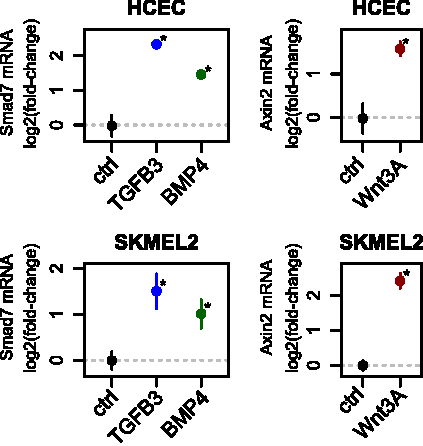
\includegraphics[width=3in]{FIGS/insulation/expression+.pdf}
  {\singlespacing 
  \caption[\tgfbsf\ and Wnt cause canonical target gene expression.]
        { The \tgf 3, Wnt3A, and BMP4 ligands cause
          expression of canonical target genes in the cell lines
          used in this dissertation. Fold-change
          is relative to the control condition. 2hr treatment. Concentrations:
          10ng/mL \tgf 3, 25ng/mL BMP4, 200ng/mL Wnt3A.
          Mean and standard deviation
          of 3 replicates, `*' indicates two-sided p-value <0.05
          (Student's t-test). mRNA levels measured by TaqMan qPCR
          (see \nameref{insulation:methods} for experimental details).
        }
  \label{fig:insulation:expression}}
  \end{figure}
  
 

  
  
\subsection{Interpretation of single-cell immunofluorescence measurements}


As for any method of measurement, it is important to
take a step back and think carefully about the biological
interpretation of the resulting data. For the image-based
single-cell data obtained in my work, cellular nuclei are
identified using Hoechst-staining and threshold segmentation,
and I only analyze those nuclei that likely belong to the G1 cell
cycle phase (see \ar{imaging:segmentation}).
Within these nuclei I tally up all pixel values to obtain
the total intensity feature, which I use as a proxy for
the quantity of the immuno-labeled target protein within the nucleus.
This feature and the mean intensity feature,
which is a proxy for concentration, are similarly informative
in my assays (\ar{fig:insulation:readoutInformation}), and
so I use the total-intensity feature for the practical
reasons described in \ar{imaging:totalIntensity}.
  

How do we interpret changes in this feature? Fold-change
over a reference (e.g. the untreated state) is a commonly used
metric, but the interpretation of fold-change is unclear in cases where
either the basal state is near zero (as any fold-change
value will move towards infinity) or is non-zero because of ``background'' signal
(which pushes all fold-change values towards 1). Using the
fluorescence image model that I present in 
\ar{imaging:model}, we can model the total intensity feature $T$
for any given nucleus $n$ by \ar{eq:system:total}. In this model the intensity of
each pixel $p$ is the sum of multiple fluorescence sources, such as
non-specific fluorescence ($F_{\text{nonspecific,}p}$,
e.g. due to off-target antibody
binding), non-signaling fluorescence ($F_{\text{nonsignaling,}p}$, 
e.g. due to a pool of the target
protein that is not involved in the studied signaling process), and the
actual signaling fluorescence $F_{\text{signaling,}p}$.
    %
    \begin{equation} \label{eq:system:total}
    T_n=\sum_p\left(F_{\text{nonspecific,}p}+F_{\text{nonsignaling,}p}+F_{\text{signaling,}p}\right)
    \end{equation}


Take the case of \bcat\ as an example. Basal
\bcat\ levels within Wnt3A-unstimulated cells are thought to be
essentially zero \arp{pathways:wnt:bcat}, and yet the measured basal levels are
quite high. This is due in large part to the presence of a
membrane-associated \bcat\ pool that does not participate in
Wnt signaling. It is impossible to know how the total nuclear
intensity breaks down into the various components of
\ar{eq:system:total}, and therefore
a metric like fold-change is uninterpretable in terms of the extent
of change for \bcat, though it can be used as a normalization method
to allow for measurements of relative change.


An alternative metric is to simply subtract a reference intensity measurement
from the experimental intensity, as the only term remaining will
be $F_\text{signaling,experiment}-F_\text{signaling,ctrl}$.
While this metric has a simple interpretation (absolute change in
signaling-associated fluorescence intensity), unfortunately it cannot be
used to infer the absolute magnitude
of response since fluorescence units are arbitrary.
Neither division nore subtraction can be used at the
single-cell level for fixed-cell assays,
as the relative contribution of each fluorescent component may vary
from cell to cell. Both metrics can be used
at the population level, however.


In summary, it is impossible to infer the absolute magnitude of change for
a signaling molecule using image-based immunofluorescence without
making assumptions that would be indefensible for the
immunofluoresce studies in this chapter. External
means of validation are then required to show that the observed
change is large enough to have a meaningful effect (as in
\ar{fig:insulation:expression}, where I show that the same experimental
treatments yield sizeable changes to target gene expression).
Relative comparisons between experimental perturbations are possible in any case,
and are easy to understand,
and so for convenience I use units normalized to a 0/1 scale throughout this chapter.


\subsection{Timepoints and concentrations}


Many studies of morphogenic signaling
pathways conflate the signal transduction and the transcriptional
decision-making processes due to use of long-term transcriptional
readouts. This conflation may be acceptable for some experimental
questions, but here my aim is to study integration specifically at
the level of signal transduction.


  \begin{figure}[!bt]
  \centering
  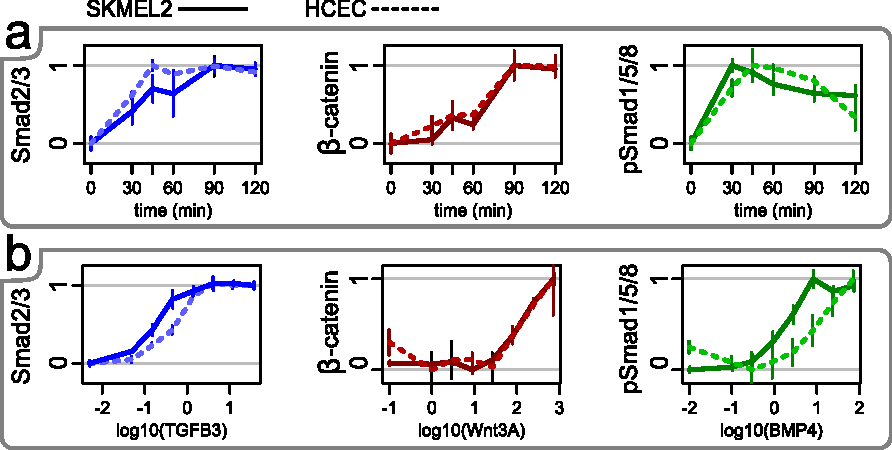
\includegraphics[width=6in]{FIGS/insulation/doseTime.pdf}
  {\singlespacing 
  \caption[Dose-response and timecourse of \tgfbsf\ and Wnt.]
        { The cell lines tested in this dissertation have similar
          but non-identical timelines (\b{a}) and
          dose-response curves (\b{b}). Shown
          are SKMEL2 (solid lines) and HCEC (dashed lines) cell lines.
          Cell lines show measurable responses between 60-120 minutes
          and are saturated by 10ng/mL \tgf 3, 1000ng/mL Wnt3A,
          or 100ng BMP4. Dose-responses are at 1hr.
          Y-axes as in \ar{fig:insulation:specificity},
          normalized so that the minimum and maximum responses
          are 0 and 1. Concentrations used in \b{a}:
		  TGFB3 (4ng/mL), Wnt3A (240ng/mL), BMP4 (70ng/mL).}
  \label{fig:insulation:doseTime}}
  \end{figure}
  

To do so, it is then necessary to minimize the effects of transcriptional
feedback on the stimulated pathways. I therefore performed
time-course experiments for each cell line and pathway in order to identify the
earliest timepoints that could still yield robust pathway responses
(shown for HCEC and SKMEL2 in \ar{fig:insulation:doseTime}a). For
all cell lines and pathways the responses were measurable by 1hr and
maximal by 2hrs, and so my crosstalk experiments take place within
this temporal window.
  

As I discuss in \ar{introduction:encodingSolution}, it is not necessarily true
that the use of a constant ligand concentration across multiple cell lines
is the appropriate way to ensure that the treatment is the ``same.'' Fortunately,
the dose-response curves for each cell line and pathway are not wildly different
(shown for HCEC and SKMEL2 in \ar{fig:insulation:doseTime}b) and so I was able
to determine concentrations that would yield approximately half-maximal responses (EC50)
or maximal responses across all cell types.


The reader may notice the use of differing ligand concentrations between
the experiments in this chapter.
For initial experiments, I did not yet know how responsive the cell types were
to each ligand, and so concentrations were based on prior work in the lab or
on literature-obtained values. For later experiments, doses were first chosen
according to whether a half-maximal or maximal response was experimentally
required, and these doses were then kept high over time to maintain saturating
levels in the face of slowly-degrading reagents and idiosyncratic sensitivities
of cell lines. Importantly, saturating concentrations
minimize the consequences of pipetting
error, since larger error can be tolerated before a measurable difference
in cellular responses will appear.

